\documentclass[../mathNotesPreamble]{subfiles}
\usetikzlibrary{external}

\providecommand{\relscalefact}{1.4}
\begin{document}
\relscale{\relscalefact}
  \section{3.1: Complex Numbers}

  \begin{defn*}[Imaginary and Complex Numbers]
    We can extend the Real numbers by defining:
      \[i=\sqrt{-1}.\]
    A \textbf{complex number} is a number of the form $a+bi$ where
    \begin{itemize}
      \item $a$ is the real part of the complex number, and
      \item $bi$ is the imaginary part of the complex number.
    \end{itemize}
    If $b=0$, then $a+bi$ is a real number.

    If $a=0$ and $b\neq 0$, then the complex number is called an \textbf{imaginary number}.

    An imaginary number is an \emph{even} root of a negative number.
  \end{defn*}

  \tikzset{external/export=false}
  \newcommand{\tikzmark}[3]{%
    \tikz[baseline=(#1.base), remember picture]%
    \node[inner sep=0pt, #3] (#1)%
    {\ensuremath{#2}};%
  }
  \begin{align*}
    \tikzmark{realPart}{5}{lander_blue}+\tikzmark{imagPart}{2i}{red!90!black}
  \end{align*}
  \begin{tikzpicture}[overlay, remember picture,
    myArrow/.style={->, shorten >=5pt, shorten <=1pt, line width=1pt}]
    \node[lander_blue] at ($(realPart.south)+(-2,-1)$) (realText) {Real part};
    \draw[myArrow, lander_blue] (realText) -- (realPart.south);
    %
    \node[red!90!black] at ($(imagPart.south)+(2,-1)$) (imagText) {Imaginary part};
    \draw[myArrow, red!90!black] (imagText) -- (imagPart.south);
  \end{tikzpicture}
  \vspace*{1.25\baselineskip}
  \tikzset{external/export=true}

  \begin{ex*}
    Express the following complex numbers in standard form:
    \begin{extasks}[after-item-skip=\stretch{1}](2)
      \task $\sqrt{-9}$
      \task $5+\sqrt{-3}$
      \task $4-\sqrt{-16}$
      \task $3-\sqrt{25}$
    \end{extasks}
    \vspace*{\stretch{1}}
  \end{ex*}
  \pagebreak

  \newcommand{\myGrid}{%
    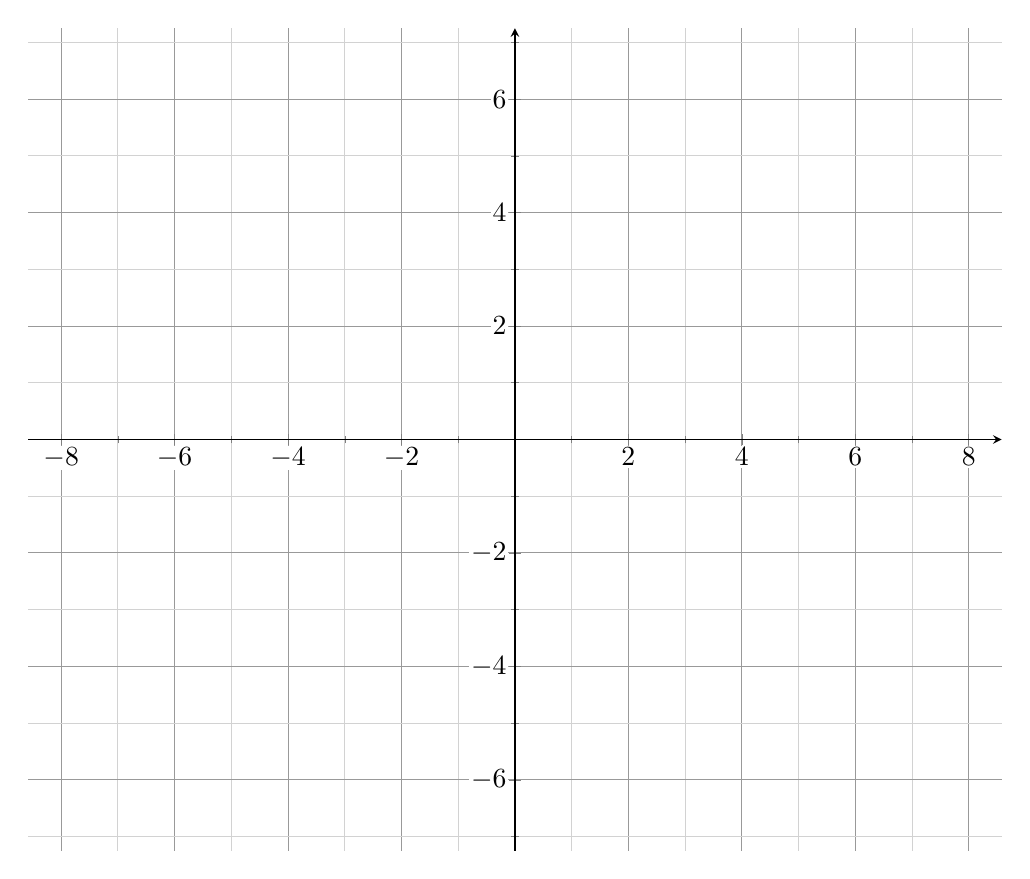
\begin{tikzpicture}
      \begin{axis}[
        grid=both, %major,minor
        grid style={line width=0.375pt, draw=gray!80},
        axis lines=center,
        axis equal,
        minor grid style={draw=gray!35},
        xmin=-7, xmax=7,
        ymin=-7.25, ymax=7.25,
        minor x tick num=1,
        minor y tick num=1,
        xtick={-8,-6,...,8},
        ytick={-8,-6,...,8},
        width=1.15\linewidth,
        enlargelimits={value=0.025, auto},
        ticklabel style={inner sep=0.75pt,fill=white,opacity=1.0, text opacity=1},
        xlabel=, ylabel=,
        every axis plot/.append style={line width=0.95pt, color=lander_blue, samples=255},
        ]
      \end{axis}
    \end{tikzpicture}
  }
  \begin{ex*}
    Graph the following complex numbers:
    \begin{extasks}[after-item-skip=\stretch{1}](2)
      \task $1+i$

        \myGrid
      \task $-2+3i$

        \myGrid
      \task $3-4i$

        \myGrid
      \task $-5-2i$

        \myGrid
    \end{extasks}
    \vspace*{\stretch{0.5}}
  \end{ex*}
  \pagebreak

  \begin{defn*}[Addition and Subtraction of complex numbers]
    Given complex numbers $a+bi$ and $c+di$,
    \begin{align*}
      \parens{a+bi}+\parens{c+di}&=\parens{a+c}+\parens{b+d}i\\[0.5\baselineskip]
      \parens{a+bi}-\parens{c+di}&=\parens{a+c}-\parens{b+d}i
    \end{align*}
  \end{defn*}
  \begin{ex*}
    Evaluate the following:
    \begin{extasks}[after-item-skip=\stretch{1}](2)
      \task $\parens{3+2i}+\parens{1-4i}$
      \task $\parens{-4-2i}-\parens{-1+5i}$
      \task $\parens{2}-\parens{-1+2i}$
      \task $\parens{5i}+\parens{3+i}$
    \end{extasks}
    \vspace*{\stretch{1}}
  \end{ex*}
  \pagebreak

  \begin{defn*}[Multiplying complex numbers]
    Given complex numbers $a+bi$ and $c+di$,
    \begin{align*}
      \parens{a+bi}\cdot\parens{c+di}&=ac+adi+bci+bdi^2\\
        &=ac+adi+bci-bd\\
        &=\parens{ac-bd}+\parens{ad+bc}i
    \end{align*}
  \end{defn*}
  \begin{ex*}
    Evaluate the following:
    \begin{extasks}[after-item-skip=\stretch{1}](2)
      \task $\parens{3+2i}\cdot\parens{1-4i}$
      \task $\parens{-4-2i}\cdot\parens{-1+5i}$
      \task $\parens{2}\cdot\parens{-1+2i}$
      \task $\parens{5i}\cdot\parens{3+i}$
    \end{extasks}
    \vspace*{\stretch{1}}
  \end{ex*}
  \pagebreak

  \begin{defn*}[Dividing complex numbers]
    Given complex numbers $a+bi$ and $c+di$, division is done via the \emph{complex conjugate}:
    \begin{align*}
      \dfrac{c+di}{a+bi}\cdot\dfrac{a-bi}{a-bi}&=\dfrac{\parens{c+di}\parens{a-bi}}{\parens{a+bi}\parens{a-bi}}\\[7.5pt]
        &=\dfrac{ac-bci+adi-bdi^2}{a^2-abi+abi-b^2i^2}\\[7.5pt]
        &=\dfrac{\parens{ac+bd}+\parens{ad-bc}i}{a^2+b^2}
    \end{align*}
  \end{defn*}
  \begin{ex*}
    Evaluate the following:
    \begin{extasks}[after-item-skip=\stretch{1}](2)
      \task $\dfrac{3+2i}{1-4i}$
      \task $\dfrac{-4-2i}{-1+5i}$
      \task $\dfrac{2}{-1+2i}$
      \task $\dfrac{3+i}{5i}$
    \end{extasks}
    \vspace*{\stretch{1}}
  \end{ex*}
  \pagebreak

  \begin{ex*}
    Given $f(x)=x^2-5x+2$, evaluate $f(3+i)$.
    \vspace*{\stretch{1}}
  \end{ex*}
  \begin{ex*}
    Given $f(x)=\dfrac{2+x}{x+3}$, evaluate $f(10i)$.
    \vspace*{\stretch{1}}
  \end{ex*}
  \pagebreak

  \begin{ex*}
    Find $i$ raised to different powers: $i$, $i^2$, $i^3$, \dots, then evaluate $i^{35}$.
  \end{ex*}

  \pagebreak
\end{document}
